%!TEX program = xelatex
\documentclass{xmu}

%%%%%%%%%%%%%%%%%%%%%%%%%%%%%%%%%%%%%%%%%%%%%%%%%%%%%%%%%%
%%%%%%%%    XMU Undergraduates Thesis Template    %%%%%%%%
%%%%%%%%             Made by: F5Soft              %%%%%%%%
%%%%%%%%  https://github.com/F5Soft/xmu-template  %%%%%%%%
%%%%%%%%%%%%%%%%%%%%%%%%%%%%%%%%%%%%%%%%%%%%%%%%%%%%%%%%%%

\begin{document}

% 电子版 / 打印版(取消注释下一行即为打印版)
\print
% 取消注释后,将在某些偶数页产生空白页,使得下一部分的内容从奇数页开始

% 取消注释后,仅使用数字作为章的编号
% \arabicchapter

% 毕业设计 / 毕业论文(取消注释下一行即为毕业设计)
% \design

% 主修 / 辅修(取消注释下一行即为辅修)
% \minor

% 标题
\title{厦门大学本科毕业论文LaTeX模版}
{An LaTeX Template of Xiamen University Undergraduate Thesis}

% 姓名
\author{F5Soft.site}

% 学号
\idn{22920182200000}

% 学院
\college{信息学院}

% 专业
\subject{计算机科学与技术}

% 年级
\grade{2018级}

% 校内指导教师
\teacher{F5Soft\; 副教授}

% 校外指导教师(注释则不显示)
\otherteacher{F5Soft\; 教授}

% 完成时间
\pubdate{二〇二二年四月三十日}

% 关键词
\keywords{本科毕业论文;LaTeX;厦门大学}
{Undergraduate Thesis; LaTeX; Xiamen University}

% 生成封面、承诺书
\maketitle

% 如果想要将致谢放在最前,可将最后的致谢移动至此

%%%%%%%% 摘要 %%%%%%%%

% 中文摘要
\begin{abstract}
    本模版基于厦门大学图书馆i学堂LaTeX讲座中提供的硕博毕业论文模版\cite{xmuischool}改编而来,并根据《厦门大学本科毕业论文(设计)规范》\cite{xmuthesis}进行了大幅度的格式调整。本模版提供高清封面、诚信承诺书、中英文摘要环境、中英文目录自动生成、附录环境、参考文献环境、致谢环境等。本模版还自带了Windows中的中易宋体、中易黑体、中易楷体、中易仿宋字体,以兼容缺少这些字体的Linux和macOS系统。
\end{abstract}

% 英文摘要
\begin{enabstract}
    This template is adapted from the master and doctoral dissertation template provided in the LaTeX lecture of Xiamen University Library i-School\cite{xmuischool}, and has been greatly adjusted according to the \textit{Xiamen University Undergraduate Thesis (Design) Specifications}\cite{xmuthesis}. This template provides high-definition cover, letter of declaration, Chinese and English abstract environment, automatic generation of table of contents in Chinese and English, appendix environment, reference environment, acknowledgements environment, etc. This template also comes with SimSun, SimHei, SimKai, and SimFang fonts in Windows to be compatible with Linux and macOS systems which lack these fonts.
\end{enabstract}

% 生成中英文目录
\tableofcontents

%%%%%%%% 正文 %%%%%%%%

\xmuchapter{使用说明}{Introduction}
\xmusection{环境配置}{Environment Setup}
首先,需要配置好LaTeX环境。这里推荐TeX Live + VSCode。其中TeX Live可访问{https://www.tug.org/texlive/}下载;VSCode安装完成后需要再搜索安装LaTeX Workshop插件。
\xmusection{编译}{Compiling}
环境配置完成后,可以从GitHub上下载本模版的代码\cite{template}。下载完成后,可尝试打开example.tex文件,点击右上角的绿色运行按钮进行编译。在macOS系统上,编译一般会失败,这是因为使用的pdflatex找不到对应中文字体的结果。可以进入左侧的LaTeX Workshop面板,选择Recipe为latexmk (xelatex),点击运行,即可编译成功。
\xmusection{使用模版}{Use Templates}
本模版根据《厦门大学本科毕业论文(设计)规范》\cite{xmuthesis}封装了大量格式设置等内容,使用时无需考虑各种格式指令,只需设置好章节标题,填充摘要、附录、参考文献、致谢等内容即可。
\xmusubsection{示例论文}{Example Paper}
example.tex文件内有详细的注释和使用示例,可以直接在该示例基础上修改。论文中的所有插图需统一放在figures文件夹内,并根据文件名来包含。
\xmusubsection{自定义模版}{Customization}
xmu.cls文件是模版文件,如果您具有排版强迫症,想和我一样对模版的细节进行微调,可以自己修改xmu.cls模版文件。模版文件中也提供了大量注释便于您进行修改。如果您认为修改的效果不错,可以在GitHub上\cite{template}发起Pull request贡献代码。您也可以发起Issue提出要添加的功能。
\par
修改模版需要有一定的LaTeX基础,可以参考《LaTeX 2e完全学习手册》\cite{latex2e}和《简单粗暴LaTeX》\cite{easylatex}中的内容进行修改。
\xmuchapter{使用示例}{Examples}
\xmusection{二级标题}{Section (English Ver.)}
一级标题(章)总会另起一页。
\xmusubsection{三级标题}{Subsection (English Ver.)}
通过xmuchapter、xmusection、xmusubsection指令指定一级(章)、二级(节)、三级(小节)标题。因为英文目录的需要,这三个指令均接收两个参数,第一个参数为中文的标题内容,第二个参数为英文的标题内容。
\subsubsection{四级标题}
如果需要四级标题的话,不会出现在目录内。
\xmusection{图表}{Figures and Tables}
\xmusubsection{插图}{Figures}
图片编号均按照章节号-图片号进行编号。可通过caption指令设置图片小标题,可通过label和ref指令引用图片编号。厦门大学校徽如下图 \ref{xmulogo} 所示。
\begin{figure}[!htb]
    \centering
    
\includegraphics[width=12em]{xmu-logo-icon.jpg}\\
    \caption{厦门大学校徽}\label{xmulogo}
\end{figure}
根据《厦门大学本科毕业论文(设计)规范》\cite{xmuthesis}要求,图片的标题和图号需要在图的下方正中位置。下面再展示一个两图并排的示例:
\begin{figure}[!htb]
    \begin{minipage}{0.5\linewidth}
        \centering
        
\includegraphics[height=5em]{xmu-logo-icon.jpg}
        \caption{厦门大学校徽}\label{xmu1}
    \end{minipage}
    \begin{minipage}{0.5\linewidth}
        \centering
        
\includegraphics[height=5em]{xmu-logo-text.jpg}
        \caption{厦门大学文字}\label{xmu2}
    \end{minipage}
\end{figure}
\xmusubsection{表格}{Tables}
对于表格,编号也按照章节号-表格号进行编号。同样可通过caption指令设置表格小标题,可通过label和ref指令引用表格编号。下表 \ref{database} 中展示了一个数据库的表设计作为示例。
\begin{table}[!htb]
    \centering
    \caption{基本资料表}
    \label{database}
    \begin{tabular}{|l|l|l|l|l|}
        \hline
        \bf\songti 字段名称 & \bf\songti 字段类型 & \bf\songti 长度 & \bf\songti 字段描述 & \bf\songti 备注 \\ \hline
        账户号             & Number          & 30            &                 & 主键            \\ \hline
        密码              & Number          & 30            & 加密              &               \\ \hline
        姓名              & Varchar         & 50            &                 &               \\ \hline
        电子邮箱            & Varchar         & 50            & VIP客户必填         &               \\ \hline
    \end{tabular}
\end{table}
根据《厦门大学本科毕业论文(设计)规范》\cite{xmuthesis}要求,表格的标题和图号需要在表的上方正中位置。表格内容的字体为5号宋体,表头的字体为5号宋体加粗。
\xmusection{画图}{Plotting}
可以使用tikzpicture环境绘制函数、折线图、散点图等,例如图 \ref{plot} 所示:
\begin{figure}[!htbp]
    \centering
    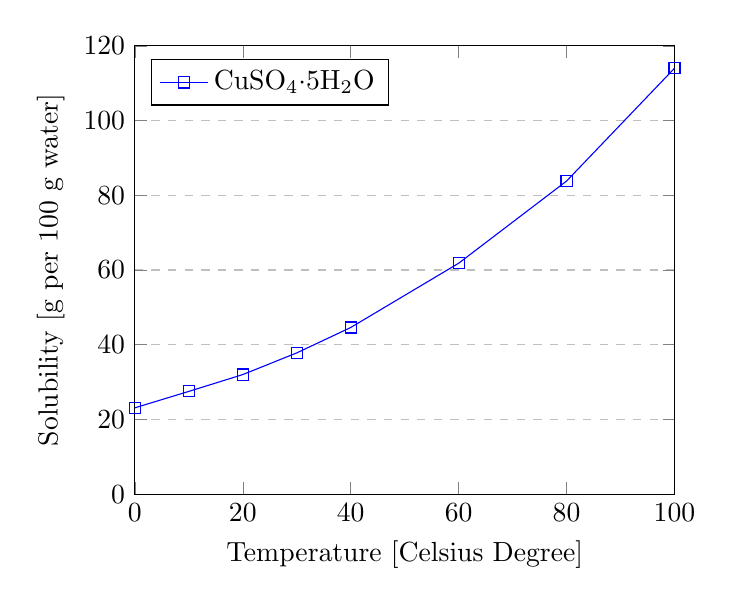
\begin{tikzpicture}
        \begin{axis}[
                xlabel={Temperature [Celsius Degree]},
                ylabel={Solubility [g per 100 g water]},
                xmin=0, xmax=100,
                ymin=0, ymax=120,
                xtick={0,20,40,60,80,100},
                ytick={0,20,40,60,80,100,120},
                legend pos=north west,
                ymajorgrids=true,
                grid style=dashed,
            ]

            \addplot[
                color=blue,
                mark=square,
            ]
            coordinates {
                    (0,23.1)(10,27.5)(20,32)(30,37.8)(40,44.6)(60,61.8)(80,83.8)(100,114)
                };
            \legend{CuSO\(_4\cdot\)5H\(_2\)O}

        \end{axis}
    \end{tikzpicture}
    \caption{Temperature dependence of CuSO\(_4\cdot\)5H\(_2\)O solubility}\label{plot}
\end{figure}
\xmusection{公式}{Formulas}
公式可以分为行内公式 $a^2+b^2=c^2$ 和行间公式:
$$
    \int_a^b\int_a^x\int_x^{x^2}(3y+7)z\;\mathrm{d}z\,\mathrm{d}y\,\mathrm{d}x
$$
$$
    |-0.75|^{2}+(5.5-4.2)^2+\sqrt[4.2]{3}+\log_{3.3}{4.7}+\cos1.24\,\sin1.7\approx5.17
$$
如果需要指定公式编号,同样可通过label和ref指令来引用。公式 \ref{eq1} 的正确结果应该为 $\frac{\sqrt{3}}{6}$。
\begin{equation}\label{eq1}
    \lim_{x\to0}\frac{\displaystyle{\int_{\sin x}^x\sqrt{3+t^2}\,\mathrm{d}t}}{x(e^{x^2}-1)}
\end{equation}
公式 \ref{eq2} 提供了一个矩阵示例,注意加粗字母最好是使用boldsymbol而非bm:
\begin{equation}\label{eq2}
    \boldsymbol{Ax} = \boldsymbol{b},\quad\boldsymbol{A} = \left(\begin{array}{ccc}
            a_{11} & a_{12} & a_{13} \\
            a_{21} & a_{22} & a_{23} \\
            a_{31} & a_{32} & a_{33} \\
        \end{array}\right),\quad \boldsymbol{b}=\left(\begin{array}{c}
            b_1 \\ b_2 \\ b_3\end{array}\right)
\end{equation}
公式 \ref{eq3} 提供了一个行列式示例:
\begin{equation}\label{eq3}
    \left|\begin{array}{cc}
        1 & 2 \\
        3 & 4 \\
    \end{array}\right|=1\times4-2\times3=-2
\end{equation}
公式 \ref{eq4} 提供了一个方程组示例:
\begin{equation}\label{eq4}
    \begin{cases}
        mgh=mv_1^2                         \\
        \dfrac12mv_2^2-\dfrac12mv_1^2=F_fs \\
        F_f=\mu mg                         \\
    \end{cases} \Rightarrow s,v_1,F_f
\end{equation}
公式字体采用的是mathptmx。
\xmusection{算法}{Algorithms}
如果只是展示代码,可考虑使用verbatim环境\footnote{更高级的代码展示可以考虑使用listings宏包中的lstlisting环境,支持代码高亮、换行、标注行号、自定义颜色、自定义字体等功能。}。
这里插入了一个脚注。可以通过footnote指令插入脚注\footnote{脚注示例。}。
\begin{verbatim}
#include <unistd.h>
int main()
{
    write(STDOUT_FILENO, "Hello, world!\n", 14);
    return 0;
}
\end{verbatim}
如果只是展示算法,而不展示具体代码,可以使用算法环境实现,例如算法 \ref{alg1}:
\begin{algorithm}[!htb]
    \KwData{sum, $i$: integer}
    \Begin{
        \For{$i\leftarrow0$ \KwTo $100$ \do}{
            sum $\leftarrow$ sum + $i$\;
            \If{\rm sum $>4000$}{
                \bf break\;
            }
        }
        \bf print \rm$i$\;
    }
    \caption{循环求和算法}\label{alg1}
\end{algorithm}

%%%%%%%% 参考文献 %%%%%%%%

\begin{reference}
    % 如果需要使用 bib 文件导入参考文献,则取消注释下一行
    % \bibliography{references.bib}
    % bib 文件可以通过百度学术、Google Scholar 的引用界面自动生成
    % 已自动按照 GB/T 7714-2005 设置参考文献的引用格式

    % 手动添加参考文献
    \begin{thebibliography}{5}
        \bibitem[1]{xmuischool} 厦门大学图书馆. i学堂直播:使用LaTeX排版论文全攻略-进阶篇[EB/OL]. \url{https://library.xmu.edu.cn/wd/jzkj/i_xt.htm}, 2021.
        \bibitem[2]{xmuthesis} 厦门大学教务处. 厦门大学本科毕业论文(设计)规范[Z]. 厦门大学教务处: 厦大教〔2016〕5号.
        \bibitem[3]{latex2e} 胡伟. LaTeX 2e完全学习手册[M]. 清华大学出版社, 2013.
        \bibitem[4]{easylatex} 吴康隆. 简单高效LaTeX[M]. 人民邮电出版社, 2020.
        \bibitem[5]{template} F5Soft.site. 厦门大学本科毕业论文LaTeX模版[EB/OL]. \url{https://github.com/F5Soft/xmu-template}, 2022.
    \end{thebibliography}
\end{reference}

%%%%%%%% 附录 %%%%%%%%

\begin{appendix}
    \xmusection{附表}{Tables}
    这里放一些附录的内容,例如表格或其他说明。如附表\ref{atable}。
    \begin{table}[!htb]
        \centering
        \caption{附表示例}
        \label{atable}
        \begin{tabular}{llr}
            \hline
            \multicolumn{2}{c}{Item} &                          \\ \cline{1-2}
            Animal                   & Description & Price (\$) \\ \hline
            Gnat                     & per gram    & 13.65      \\
                                     & each        & 0.01       \\
            Gnu                      & stuffed     & 92.50      \\
            Emu                      & stuffed     & 33.33      \\
            Armadillo                & frozen      & 8.99       \\ \hline
        \end{tabular}
    \end{table}
    附录中的编号均以字母A开头。例如公式 \ref{eq5}
    \begin{equation}\label{eq5}
        \sin \left(2x+\frac\pi2\right)=\frac 12
    \end{equation}
    \xmusection{厦门大学本科毕业论文(设计)规范摘要}{Abstract of Xiamen University Undergraduate Dissertation (Design) Specification}
    主修专业毕业论文(设计)封面使用 160g 白色双胶纸,辅修封面为 160g 浅黄色皮纹纸。内页均为 A4 规格 80g 双胶纸。\par
    章的标题占2行,标题以外的文字为1.5倍行距。\par
    上边距和左边距应留 25mm 以上间隙,下边距和右边距应分别留 20mm 以上间隙。\par
    每页须加“页眉”和“页码”。奇数页页眉内容为当前章名,如“第一章 绪论”。偶数页页眉内容为论文题目。学位论文的页码,正文、参考文献、附录部分用阿拉伯数字连续编码并居中,前置部分用罗马数字单独连续编码居中(封面除外)。\par
    封面中文标题:二号黑体\par
    封面英文标题:三号 Times New Roman 加粗\par
    中文摘要标题:小三号黑体\par
    中文关键词标题:小四号黑体\par
    中文摘要、关键词内容:小四号宋体\par
    英文摘要标题:小三号 Times New Roman 加粗\par
    英文关键词标题:小四号 Times New Roman 加粗\par
    英文摘要、关键词内容:小四号 Times New Roman\par
    中文目录标题:小三号黑体\par
    中文目录中章的标题:四号黑体\par
    中文目录中节的标题:小四号黑体\par
    中文目录中三级标题:小四号宋体\par
    英文目录标题:小三号 Times New Roman 加粗\par
    英文目录中章的标题:四号 Times New Roman 加粗\par
    英文目录中节的标题:小四号 Times New Roman 加粗\par
    英文目录中三级标题:小四号 Times New Roman\par
    章的标题:小三号黑体\par
    节的标题:四号黑体\par
    三级标题:小四号黑体\par
    正文:小四号宋体\par
    页眉:小五号宋体\par
    页码:小五号 Times New Roman\par
    注释内容:小五号宋体\par
    表格、图的标题、单位、表头:五号宋体加粗\par
    表格内容:五号宋体\par
    表格、图的资料来源:小五号宋体\par
    参考文献标题:小三号黑体\par
    中文参考文献表:五号宋体\par
    英文参考文献表:五号 Times New Roman\par
    附录标题:小三号黑体\par
    致谢标题:小三号黑体\par
    致谢内容:小四号宋体\par
    对于中英文混杂的内容,{\bf\songti 中文的字体若是用宋体,英文的字体则采用Times New Roman};{\sf 中文的字体若是黑体,英文的字体则采用Arial}。\footnote{
        因此,本模版提供了如下的几种字体设置。rm:罗马字族,中文宋体,英文Times。sf:等线字族,中文黑体,英文Arial。bf:粗体序列,中文黑体,英文Times加粗。it:斜体序列,中文楷体,英文Times斜体。如果需要使用难看的宋体加粗,则需要通过 \textbackslash bf\textbackslash songti实现。当然,也可以使用 songti、heiti、kaishu 手动指定中文字体,此时英文字体均默认为Times。
    }
    \xmusubsection{附录三级标题}{Subsection in Appendix}
    \subsubsection{附录四级标题}
\end{appendix}

%%%%%%%% 致谢(默认在最后) %%%%%%%%

\begin{acknowledgement}
    虽然在《厦门大学本科毕业论文(设计)规范》中,致谢应放在前置部分,但是正常情况下致谢应该几乎都是放在最后的。
    \par
    《规范》中还强调,致谢语应以简短的文字对课题研究与论文撰写过程中曾直接给予帮助的人员(例如指导教师、答疑教师及其他人员)表示自己的谢意。所以如果本模版对你的毕业论文有帮助的话,可以尝试将其写到致谢中。
\end{acknowledgement}

\end{document}
